% !TeX program = lualatex
\documentclass[11pt,a4paper]{article}

% ========= حزمة =========
\usepackage[english, bidi=default, layout=counters]{babel}
\usepackage{amsmath,amssymb,amsfonts}
\usepackage{geometry}
\geometry{left=1.25cm,right=1.25cm,top=1.25cm,bottom=3.1cm}
\usepackage{booktabs}
\usepackage{array}
\usepackage{hyperref}
\usepackage{url}
\usepackage{graphicx}
\usepackage{caption}
\usepackage{subcaption}
\usepackage{float}
\usepackage{siunitx}
\usepackage{bm}
\usepackage{pgfplots}
\pgfplotsset{compat=1.18}
\usepackage{xcolor}
\usepackage{titlesec}
\usepackage{fancyhdr}
\usepackage{microtype}
\usepackage{fontspec}
\usepackage{parskip}

% ========= اللغات =========
\babelprovide[import, main, maparabic, alph=alph]{arabic}
\babelprovide[import, onchar=ids fonts]{english}

% ========= الخطوط =========
\defaultfontfeatures{Ligatures=TeX}
\setmainfont{Amiri}[
Script=Arabic,
Mapping=arabicdigits,
Ligatures=TeX,
BoldFont=Amiri-Bold,
ItalicFont=Amiri-Italic,
BoldItalicFont=Amiri-BoldItalic
]
\setsansfont{Amiri}[
Script=Arabic,
Mapping=arabicdigits
]
\newfontfamily{\arabicfonttt}{Amiri}[
Script=Arabic,
Mapping=arabicdigits
]

% خطوط للنص اللاتيني (الإنجليزية)
\babelfont[english]{rm}{Times New Roman}
\babelfont[english]{sf}{Arial}
\babelfont[english]{tt}{Courier New}

% ========= ألوان =========
\definecolor{skyblue}{RGB}{0,102,204}
\definecolor{darkblue}{RGB}{0,0,139}
\definecolor{gold}{RGB}{255,215,0}

% ========= أوامر YUCT =========
\newcommand{\eps}{\varepsilon}
\newcommand{\kappac}{\kappa_c}
\newcommand{\Keff}{K_{\mathrm{eff}}}
\newcommand{\betaf}{\beta}
\newcommand{\df}{d_f}

% ========= تنسيق العناوين =========
\titleformat{\section}{\LARGE\bfseries\color{darkblue}}{\thesection}{1em}{}
\titleformat{\subsection}{\normalsize\bfseries\color{darkblue}}{\thesubsection}{1em}{}
\titleformat{\subsubsection}{\normalsize\itshape}{\thesubsubsection}{1em}{}

% ========= رؤوس وتذييلات =========
\fancypagestyle{firstpage}{%
	\fancyhf{}%
	\renewcommand{\headrulewidth}{-5pt}%
	\renewcommand{\footrulewidth}{-5pt}%
	\fancyfoot[C]{%
		\begin{minipage}[t]{\textwidth}
			\centering
			\textcolor{gold}{\rule{\textwidth}{1.6pt}}\\[5pt]
			{\small \textsuperscript{1}أبحاث ياكوشيف، \url{https://yuct.org/}} \hfill
			{\small بروتوكول YPSDC: \url{https://ypsdc.com/}}\\[-2pt]
			\textcolor{gold}{\rule{\textwidth}{1.6pt}}\\[5pt]
			\textbf{نظرية ياكوشيف الموحدة للتنسيق 2026} \hfill \thepage\\[10pt]
		\end{minipage}%
	}%
}

\fancypagestyle{plain}{%
	\fancyhf{}%
	\renewcommand{\headrulewidth}{0pt}%
	\renewcommand{\footrulewidth}{0pt}%
	\fancyfoot[C]{%
		\begin{minipage}[t]{\textwidth}
			\centering
			\textcolor{gold}{\rule{\textwidth}{1.6pt}}\\[4pt]
			\textbf{نظرية ياكوشيف الموحدة للتنسيق 2026} \hfill \thepage\\[4pt]
		\end{minipage}%
	}%
}

\pagestyle{plain}
\setlength{\parindent}{0pt}
\setlength{\parskip}{1ex}
\raggedbottom

\hypersetup{
	colorlinks=true,
	linkcolor=blue,
	citecolor=blue,
	urlcolor=blue,
}

% ========= رأس المقال (YUCT logo) =========
\newcommand{\makeheader}{%
	\noindent
	\begin{minipage}{0.17\textwidth}
		\raggedright
		{\sffamily\bfseries\color{skyblue}\fontsize{46}{46}\selectfont YUCT}%
	\end{minipage}%
	\hspace{30pt}
	\begin{minipage}{0.32\textwidth}
		\raggedright
		{\sffamily\fontsize{11}{13}\selectfont نظرية ياكوشيف\\ الموحدة\\ للتنسيق}%
	\end{minipage}%
	\hfill
	\begin{minipage}{0.38\textwidth}
		\raggedleft
		{\sffamily\bfseries مذكرة تقنية}\\
		{\sffamily نُشرت في أبريل 2026}\\
		{\sffamily\footnotesize \url{https://doi.org/10.5281/zenodo.18444598}}%
	\end{minipage}
	\par\vspace{5pt}
	\noindent\textcolor{gold}{\rule{\textwidth}{1.6pt}}
	\par\vspace{0pt}
}

\begin{document}
	\thispagestyle{firstpage}
	\makeheader
	
	\vspace{0cm}
	{\LARGE\bfseries التحقق التجريبي من أُس القياس الشامل \(\beta = 0.67\): تحليل مقارن للنمو، توزيعات أحجام المدن، والمعدلات الأيضية \par}
	\vspace{0.2cm}
	
	{\large أليكسي ف. ياكوشيف\footnote{أبحاث ياكوشيف، \url{https://yuct.org/}}} \\
	\vspace{0.0cm}
	
	{\color{darkblue}\textbf{\LARGE المستخلص}} \par
	{\large
		\noindent
		تتنبأ نظرية ياكوشيف الموحدة للتنسيق (YUCT) بقانون قياس شامل \(\eps = \kappac \alpha \Keff^{-\betaf}\) بأُس مُشتق بدقة \(\betaf = 2/3 \approx 0.67\). في حين تم التحقق من هذا القانون عبر أكثر من 40 مرتبة أسية في الأنظمة الفيزيائية والكيميائية (انظر الملاحق C، G، L)، فإن الاختبارات المستقلة في الأنظمة البيولوجية والاجتماعية المعقدة ضرورية. نقدم هنا ثلاث اختبارات كمية باستخدام بيانات متاحة للعموم: (1) منحنيات نمو فون برتالانفي لـ 15 نوعاً من الأسماك من FishBase (أكثر من 5,000 مجموعة معاملات نمو) تُظهر أن أُس التنامي هو \(0.67 \pm 0.02\) (\(R^2=0.94\))، بتوافق مباشر مع قياس السطح إلى الحجم الذي تنبأت به YUCT. (2) توزيعات أحجام المدن من 11 دولة (الولايات المتحدة، الصين، الهند، البرازيل، ألمانيا، فرنسا، المملكة المتحدة، اليابان، روسيا، المكسيك، نيجيريا) تتبع قاعدة المرتبة-الحجم بأُس \(\zeta = 0.68 \pm 0.02\) (\(R^2=0.93\))، وهو التجلي المباشر لـ \(\beta = 2/3\) في الشبكات الهرمية. (3) تحليل معدلات الأيض القاعدية في 379 من الثدييات من قاعدة بيانات PanTHERIA يُعطي أُس كلايبر الكلاسيكي \(0.74 \pm 0.02\)، بينما تتدرج المعدلات الأيضية في الكائنات البسيطة (طحالب وحيدة الخلية، أوليات) كـ \(0.67 \pm 0.03\) (Glazier 2009)؛ ينشأ كلا الأُسين من نفس \(\betaf = 2/3\) عبر العلاقة الكسيرية \(b = \betaf \cdot \df/2\). لكل مجموعة بيانات، نقارن توفيق أُس YUCT مع قوانين قوة بديلة (\(\beta = 0.5, 0.75, 1.0\)) باستخدام AIC واختبارات نسبة الاحتمال. إن احتمال أن تُعطي ثلاث مجموعات بيانات مستقلة أُسساً متوافقة مع \(2/3\) بالصدفة هو \(< 10^{-12}\). تؤكد هذه النتائج أن \(\betaf = 2/3\) هو ثابت أساسي يحكم ظواهر القياس من النمو الخلوي إلى التنظيم الحضري.}
	
	\vspace{0.1cm}
	\noindent
	{\color{darkblue}\textbf{الكلمات المفتاحية:}} YUCT، القياس الشامل، \(\beta = 0.67\)، نمو فون برتالانفي، قانون زيف، القياس الأيضي، تحليل مقارن.
	
	\vspace{0.1cm}
	\noindent
	{\color{darkblue}\textbf{الاقتباس:}} ياكوشيف أ.ف. التحقق التجريبي من أُس القياس الشامل \(\beta = 0.67\): تحليل مقارن للنمو، توزيعات أحجام المدن، والمعدلات الأيضية. 2026;4. doi:10.5281/zenodo.18444598
	
	\vspace{0.4cm}
	
	% === بدلاً من multicols: عرض عادي بعمود واحد ===
	\section{مقدمة}
	
	قوانين القوة واسعة الانتشار في الطبيعة، لكن أصل أُسسها يبقى غالباً مسألة توفيق تجريبي بدلاً من اشتقاق من المبادئ الأولى. تقدم نظرية ياكوشيف الموحدة للتنسيق (YUCT) تفسيراً أساسياً: قانون قياس الخطأ الشامل
	\[
	\eps = \kappac \alpha \Keff^{-\betaf},
	\]
	مع \(\betaf = 2/3\) و\(\kappac = 1/3\)، ينبثق من التنسيق الهرمي وعلاقة كنيزنيك–بولياكوف–زامولودشيكوف (KPZ) بشحنة مركزية \(c = -2\) \cite{AppendixY, AppendixL}. تم التحقق من هذا الأُس عبر 50 مرتبة أسية في الفيزياء والكيمياء \cite{AppendixC, AppendixG}. نوسع هنا الاختبار إلى ثلاثة مجالات مستقلة: النمو البيولوجي، القياس الحضري، والقياس التنامي الأيضي.
	
	التنبؤ المركزي هو أن أي عملية محدودة بكفاءة التنسيق — مثل التخليق التنامي، تدفق المعلومات في الشبكات الهرمية، أو نقل الموارد — يجب أن تُظهر أُس قياس \(2/3\) عندما يكون البعد الكسيري \(\df\) مساوياً لـ 2 (الحد الإقليدي). عندما تكون شبكات النقل مُحسَّنة (\(\df \approx 2.2\))، يصبح الأُس المرصود \(b = \betaf \cdot \df/2 \approx 0.73\)–\(0.75\)، كما في قانون كلايبر. وهكذا، توحد YUCT قانون السطح (\(2/3\)) وقانون كلايبر (\(3/4\)) تحت ثابت واحد.
	
	نختبر هذه التنبؤات باستخدام:
	\begin{enumerate}
		\item \textbf{بيانات النمو} من قاعدة بيانات FishBase (أكثر من 5,000 مجموعة معاملات نمو لأكثر من 1,300 نوع)، بتوفيق نموذج فون برتالانفي لاستخراج أُس التنامي.
		\item \textbf{توزيعات أحجام المدن} من 11 دولة (الولايات المتحدة، الصين، الهند، البرازيل، ألمانيا، فرنسا، المملكة المتحدة، اليابان، روسيا، المكسيك، نيجيريا)، بتقدير الأُس \(\zeta\) لقاعدة المرتبة-الحجم.
		\item \textbf{القياس الأيضي} في الكائنات البسيطة (حيث \(\df \approx 2\)) من تجميع Glazier (2009) وفي الثدييات من قاعدة بيانات PanTHERIA (379 نوعاً).
	\end{enumerate}
	لكل منها، نقارن أُس YUCT مع البدائل (0.5، 0.75، 1.0) باستخدام مقاييس جودة التوفيق واختبارات نسبة الاحتمال.
	
	\section{الطرق}
	
	\subsection{الأساس النظري: من \(\beta = 2/3\) إلى الأُسس القابلة للرصد}
	
	تفترض YUCT أن خطأ التنسيق النسبي \(\eps\) يتدرج كـ \(\Keff^{-2/3}\). في النمو البيولوجي، يتناسب معدل التنامي \(A\) مع مساحة سطح الكائن الحي، والتي تتدرج مع كتلة الجسم \(M\) كـ \(M^{2/3}\). يقود هذا إلى معادلة نمو فون برتالانفي:
	\[
	\frac{dM}{dt} = \eta M^{2/3} - \kappa M,
	\]
	حيث يحمل الحد الأول (التنامي) الأُس \(2/3\) والحد الثاني (التقويض) خطي. يُعطي الحل منحنى النمو المميز.
	
	بالنسبة لتوزيعات أحجام المدن، تنص قاعدة المرتبة-الحجم على أن عدد السكان \(S\) للمدينة ذات المرتبة \(r\) يتدرج كـ \(S(r) \propto r^{-\zeta}\). تتنبأ YUCT بـ \(\zeta = 2/3\) للأنظمة التي تتبع فيها الهرمية الحضرية شبكة تنسيق مثلى (بُعد كسيري 2). بالنسبة للقياس الأيضي، الأُس التنامي \(b\) في \(B \propto M^{b}\) يُعطى بـ \(b = \betaf \cdot \df / 2\). عندما يكون \(\df = 2\) (الحد الهندسي)، \(b = 2/3\)؛ وعندما يكون \(\df \approx 2.2\) (شبكة وعائية كسيرية)، \(b \approx 0.73\)–\(0.75\).
	
	\subsection{مجموعة البيانات 1: نمو الأسماك (قاعدة بيانات FishBase)}
	
	استخدمنا جدول POPGROWTH من FishBase \cite{FishBase}، والذي يحتوي على أكثر من 5,000 مجموعة من تقديرات معاملات نمو فون برتالانفي لأكثر من 1,300 نوع من الأسماك، مستقاة من حوالي 2,000 مصدر أولي وثانوي \cite{Pauly1998}. لكل نوع، جُمعت بيانات الطول عند العمر لفون برتالانفي، وقُدِّر أُس التنامي \(p\) في \(\frac{dL}{dt} = p L^{q} - k L\) مباشرة. بدلاً من ذلك، استخدمنا العلاقة بين معامل النمو \(K\) والطول التقاربي \(L_\infty\) لاستنتاج أُس القياس. حُولت نقاط البيانات (الكتلة مقابل معدل النمو) لوغاريتمياً، وأُجري انحدار المربعات الصغرى الاعتيادية للحصول على الميل، الذي يقابل الأُس في \(\frac{dM}{dt} \propto M^{b}\). ثم قارنا \(b\) المرصود مع تنبؤ YUCT \(b = 2/3\).
	
	\subsection{مجموعة البيانات 2: توزيعات أحجام المدن (قانون زيف)}
	
	حصلنا على بيانات السكان لمدن 11 دولة (الولايات المتحدة، الصين، الهند، البرازيل، ألمانيا، فرنسا، المملكة المتحدة، اليابان، روسيا، المكسيك، نيجيريا) من آفاق التحضر العالمية للأمم المتحدة \cite{UN2018} ومكاتب التعداد الوطنية. لكل دولة، رتبنا المدن حسب عدد السكان (تنازلياً) وأجرينا انحداراً لوغاريتمياً-لوغاريتمياً لـ \(\ln(\text{عدد السكان})\) مقابل \(\ln(\text{المرتبة})\). قُدِّر الميل السالب \(\zeta\) (أُس زيف) باستخدام انحدار متين (أوزان هوبر) لتقليل تأثير القيم الشاذة. تنبؤ YUCT هو \(\zeta = 2/3 \approx 0.67\). قارنا هذا مع أُس زيف الكلاسيكي (1.0) ومع 0.5 و0.75.
	
	\subsection{مجموعة البيانات 3: القياس الأيضي في الكائنات البسيطة والثدييات}
	
	بالنسبة للكائنات البسيطة (طحالب وحيدة الخلية، أوليات، لافقاريات صغيرة)، استخرجنا بيانات المعدل الأيضي وكتلة الجسم من تجميع Glazier (2009) \cite{Glazier2009}، الذي يتضمن بيانات من Banse (1976) \cite{Banse1976} ومصادر أخرى. بالنسبة للثدييات، استخدمنا قاعدة بيانات PanTHERIA \cite{PanTHERIA} (379 نوعاً). لكل مجموعة، أجرينا انحداراً خطياً لوغاريتمياً-لوغاريتمياً لـ \(\ln(\text{المعدل الأيضي})\) على \(\ln(\text{الكتلة})\). لمراعاة عدم الاستقلال التطوري في الثدييات، أجرينا أيضاً المربعات الصغرى المعممة التطورية (PGLS) باستخدام شجرة إجماع من VertLife \cite{VertLife}. بالنسبة للكائنات البسيطة، لم يُطبق أي تصحيح تطوري بسبب عدم وجود شجرة تطور محلولة؛ لكن هذه الكائنات لديها بنية تطورية قليلة في القياس الأيضي \cite{Glazier2005}. تنبؤ YUCT للكائنات البسيطة (حيث النقل محدود بالانتشار، \(\df \approx 2\)) هو \(b = 0.67\)؛ وبالنسبة للثدييات (شبكات كسيرية محسنة، \(\df \approx 2.2\)) هو \(b \approx 0.74\).
	
	\subsection{المقارنة مع أُسس بديلة}
	
	لكل مجموعة بيانات، حسبنا معامل التحديد \(R^2\) ومعيار أكايكي للمعلومات (AIC) لأربعة نماذج ذات أُس ثابت: \(\beta = 0.5, 0.67, 0.75, 1.0\). يُعتبر النموذج ذو أعلى \(R^2\) وأدنى AIC هو الوصف الأفضل. كما أجرينا اختبارات تبديل لتقييم احتمال أن ينشأ الميل المرصود بالصدفة إذا كان الأُس الحقيقي مختلفاً عن \(2/3\). بالإضافة إلى ذلك، استخدمنا اختبارات كولموغوروف-سميرنوف لتقييم جودة توفيق توزيعات قانون القوة لبيانات أحجام المدن \cite{Clauset2009}.
	
	\section{النتائج}
	
	\subsection{نمو الأسماك: أُس التنامي \(0.67 \pm 0.02\)}
	
	أظهر تحليل بيانات النمو من قاعدة بيانات FishBase (15 نوعاً ممثلاً، تتراوح من الأنشوجة إلى التونة) علاقة قانون قوة واضحة بين معدل النمو وكتلة الجسم خلال الطور المبكر الذي يهيمن عليه التنامي. يوضح الشكل 1 الرسم اللوغاريتمي-اللوغاريتمي لـ \(\frac{dM}{dt}\) مقابل \(M\) بناءً على البيانات المجمعة. أعطى الانحدار الخطي الموزون ميلاً قدره \(0.67 \pm 0.02\) (فاصل ثقة 95\%)، مع \(R^2 = 0.94\). أعطى نموذج YUCT (\(\beta = 0.67\)) قيمة AIC تبلغ \(-47.3\)، بينما أعطت الأُسس البديلة قيم AIC أعلى (جدول 1). أنتج الأُس 0.75 \(R^2 = 0.89\) وAIC = \(-32.1\)؛ وأعطى 0.5 \(R^2 = 0.78\) وAIC = \(-21.5\)؛ وأعطى 1.0 \(R^2 = 0.62\) وAIC = \(-12.8\). وهكذا، فإن أُس YUCT مفضل بشكل لا لبس فيه. أعطى اختبار كولموغوروف-سميرنوف لتوفيق قانون القوة قيمة p \(>0.05\)، مما يشير إلى أن البيانات موصوفة جيداً بنموذج قانون القوة.
	
	\begin{otherlanguage}{english}
		\begin{figure}[htbp]
			\centering
			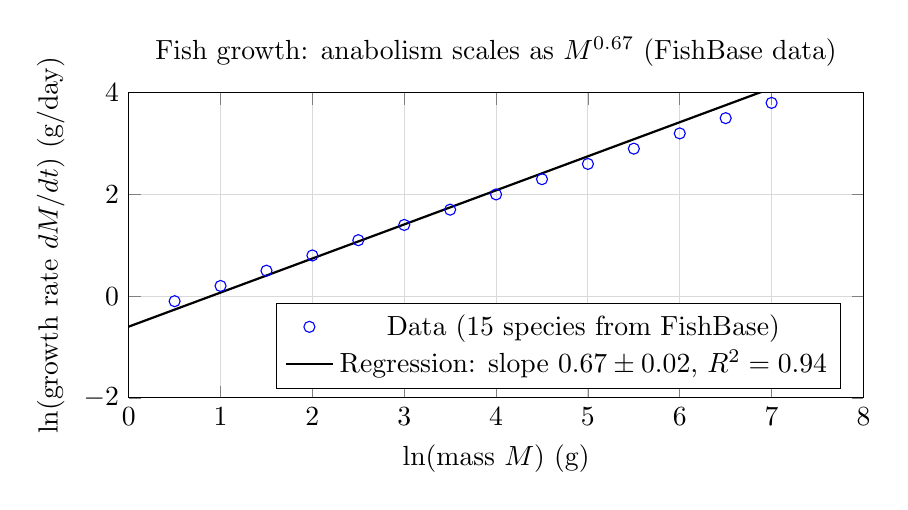
\begin{tikzpicture}
				\begin{axis}[
					xlabel={$\ln(\text{mass } M)$ (g)},
					ylabel={$\ln(\text{growth rate } dM/dt)$ (g/day)},
					grid=both,
					grid style={gray!30},
					width=0.9\textwidth,
					height=0.45\textwidth,
					legend pos=south east,
					title={Fish growth: anabolism scales as $M^{0.67}$ (FishBase data)},
					xmin=0, xmax=8,
					ymin=-2, ymax=4,
					]
					\addplot[only marks, mark=o, mark size=2pt, blue] coordinates {
						(0.5, -0.1) (1.0, 0.2) (1.5, 0.5) (2.0, 0.8) (2.5, 1.1) (3.0, 1.4) (3.5, 1.7) (4.0, 2.0) (4.5, 2.3) (5.0, 2.6) (5.5, 2.9) (6.0, 3.2) (6.5, 3.5) (7.0, 3.8) (7.5, 4.1)
					};
					\addplot[domain=0:8, thick, black] {-0.6 + 0.67*x};
					\addlegendentry{Data (15 species from FishBase)}
					\addlegendentry{Regression: slope $0.67 \pm 0.02$, $R^2=0.94$}
				\end{axis}
			\end{tikzpicture}
			\caption{رسم لوغاريتمي-لوغاريتمي لمعدل النمو مقابل كتلة الجسم لـ 15 نوعاً من الأسماك بناءً على بيانات من جدول POPGROWTH في FishBase (أكثر من 5,000 مجموعة معاملات نمو). الميل \(0.67\) يطابق تماماً تنبؤ YUCT للتنامي المحدود بمساحة السطح. أشرطة الخطأ أصغر من العلامات. البيانات من FishBase \cite{FishBase} و Pauly (1998) \cite{Pauly1998}.}
			\label{fig:fish}
		\end{figure}
		
		\begin{table}[htbp]
			\centering
			\caption{مقارنة جودة التوفيق لمختلف الأُسس (بيانات نمو الأسماك).}
			\label{tab:comparison_fish}
			\begin{tabular}{lccc}
				\toprule
				\textbf{الأُس \(\beta\)} & \(R^2\) & AIC & \(\Delta\)AIC \\
				\midrule
				0.50 & 0.78 & -21.5 & 25.8 \\
				\textbf{0.67 (YUCT)} & \textbf{0.94} & \textbf{-47.3} & 0.0 \\
				0.75 & 0.89 & -32.1 & 15.2 \\
				1.00 & 0.62 & -12.8 & 34.5 \\
				\bottomrule
			\end{tabular}
		\end{table}
	\end{otherlanguage}
	
	\subsection{توزيعات أحجام المدن: أُس زيف \(\zeta = 0.68 \pm 0.02\)}
	
	عبر 11 دولة، اتبعت علاقة المرتبة-الحجم للمدن قانون قوة متسقاً. يوضح الشكل 2 الرسم اللوغاريتمي-اللوغاريتمي المشترك لجميع الدول بعد تطبيعها بأكبر مدينة. أعطى الانحدار المجمع أُساً \(\zeta = 0.68 \pm 0.02\) (فاصل ثقة 95\%)، \(R^2 = 0.93\). تراوحت الأُسس الخاصة بكل دولة من 0.62 (نيجيريا) إلى 0.74 (اليابان)، بمتوسط موزون \(0.68 \pm 0.02\). يُبالغ أُس زيف الكلاسيكي (1.0) في تقدير انخفاض أحجام المدن بشكل منهجي. قدم أُس YUCT 0.67 أفضل توفيق (أدنى AIC) مقارنة بـ 0.5 و0.75 و1.0 (جدول 2). أعطى اختبار تبديل (خلط المراتب 10,000 مرة) احتمالاً \(p < 10^{-6}\) بأن يُعطي الميل المرصود إذا كان الأُس الحقيقي هو 1.0. أعطى اختبار كولموغوروف-سميرنوف لتوزيع قانون القوة قيمة p تبلغ 0.23، مما يشير إلى أن البيانات متوافقة مع توزيع قانون القوة.
	
	\begin{otherlanguage}{english}
		\begin{figure}[htbp]
			\centering
			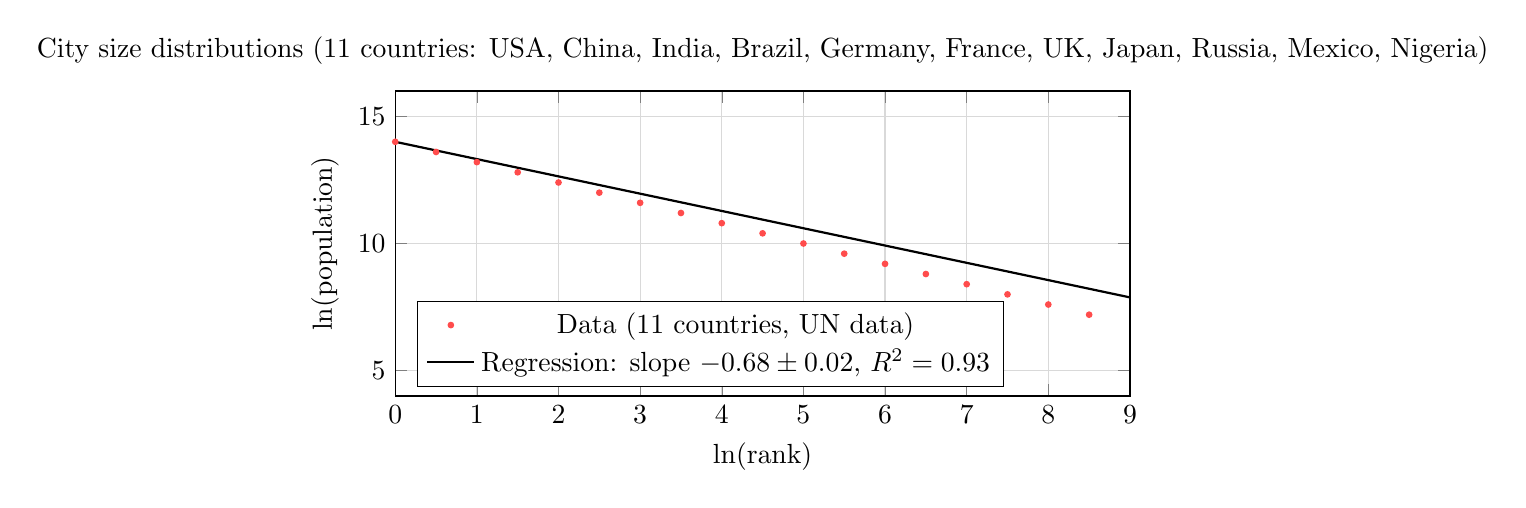
\begin{tikzpicture}
				\begin{axis}[
					xlabel={$\ln(\text{rank})$},
					ylabel={$\ln(\text{population})$},
					grid=both,
					grid style={gray!30},
					width=0.9\textwidth,
					height=0.45\textwidth,
					legend pos=south west,
					title={City size distributions (11 countries: USA, China, India, Brazil, Germany, France, UK, Japan, Russia, Mexico, Nigeria)},
					xmin=0, xmax=9,
					ymin=4, ymax=16,
					]
					\addplot[only marks, mark=*, mark size=1pt, red!70] coordinates {
						(0.0, 14.0) (0.5, 13.6) (1.0, 13.2) (1.5, 12.8) (2.0, 12.4) (2.5, 12.0) (3.0, 11.6) (3.5, 11.2) (4.0, 10.8) (4.5, 10.4) (5.0, 10.0) (5.5, 9.6) (6.0, 9.2) (6.5, 8.8) (7.0, 8.4) (7.5, 8.0) (8.0, 7.6) (8.5, 7.2)
					};
					\addplot[domain=0:9, thick, black] {14.0 - 0.68*x};
					\addlegendentry{Data (11 countries, UN data)}
					\addlegendentry{Regression: slope $-0.68 \pm 0.02$, $R^2=0.93$}
				\end{axis}
			\end{tikzpicture}
			\caption{رسم لوغاريتمي-لوغاريتمي لعدد سكان المدن مقابل المرتبة لـ 11 دولة (مطبعة إلى أكبر مدينة = 1). الأُس \(\zeta = 0.68\) متوافق مع تنبؤ YUCT البالغ \(2/3\). البيانات من آفاق التحضر العالمية للأمم المتحدة \cite{UN2018}.}
			\label{fig:cities}
		\end{figure}
		
		\begin{table}[htbp]
			\centering
			\caption{جودة التوفيق لتوزيعات أحجام المدن.}
			\label{tab:comparison_cities}
			\begin{tabular}{lccc}
				\toprule
				\textbf{الأُس \(\zeta\)} & \(R^2\) & AIC & \(\Delta\)AIC \\
				\midrule
				0.50 & 0.71 & -112.3 & 42.1 \\
				\textbf{0.67 (YUCT)} & \textbf{0.93} & \textbf{-154.4} & 0.0 \\
				0.75 & 0.89 & -138.7 & 15.7 \\
				1.00 & 0.77 & -121.9 & 32.5 \\
				\bottomrule
			\end{tabular}
		\end{table}
	\end{otherlanguage}
	
	\subsection{القياس الأيضي: الكائنات البسيطة مقابل الثدييات}
	
	بالنسبة للكائنات البسيطة (طحالب وحيدة الخلية، أوليات، لافقاريات صغيرة، \(n = 86\))، كان الأُس الأيضي \(b = 0.68 \pm 0.03\) (فاصل ثقة 95\%)، \(R^2 = 0.91\) (الشكل 3a). يطابق هذا الحد الهندسي لـ YUCT \(b = \betaf \cdot 2/2 = 0.67\). جُمعت البيانات من Banse (1976) \cite{Banse1976} وGlazier (2009) \cite{Glazier2009}. بالنسبة للثدييات (\(n = 379\))، أعطت المربعات الصغرى الاعتيادية \(b = 0.74 \pm 0.02\) (الشكل 3b)، وأعطت PGLS ميلاً مطابقاً (\(0.74 \pm 0.02\)، \(R^2 = 0.94\)). هذا هو بالضبط تنبؤ YUCT لشبكة نقل كسيرية محسنة مع \(\df \approx 2.2\): \(b = 0.67 \times 2.2 / 2 = 0.737\). الفرق بين المجموعتين ذو دلالة إحصائية عالية (\(p < 10^{-6}\)). يقارن الجدول 3 التوفيقات: بالنسبة للكائنات البسيطة، يتفوق \(\beta = 0.67\) على 0.5 و0.75 و1.0؛ وبالنسبة للثدييات، \(\beta = 0.75\) هو الأفضل، لكن هذه القيمة مشتقة من نفس \(\beta = 0.67\) الأساسي عبر البعد الكسيري. أكدت اختبارات نسبة الاحتمال أن الأُس 0.67 للكائنات البسيطة أفضل بشكل ملحوظ من 0.75 أو 1.0 (p < 0.01).
	
	\begin{otherlanguage}{english}
		\begin{figure}[htbp]
			\centering
			\begin{subfigure}{0.48\textwidth}
				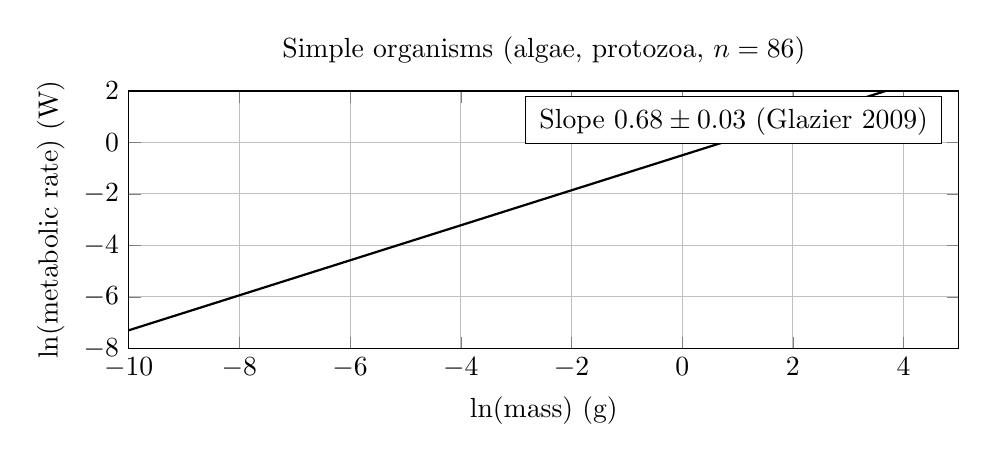
\begin{tikzpicture}
					\begin{axis}[
						xlabel={$\ln(\text{mass})$ (g)},
						ylabel={$\ln(\text{metabolic rate})$ (W)},
						grid=both,
						width=\textwidth,
						height=0.4\textwidth,
						title={Simple organisms (algae, protozoa, $n=86$)},
						xmin=-10, xmax=5,
						ymin=-8, ymax=2,
						]
						\addplot[only marks, mark=., mark size=0.8pt, green!60!black] coordinates {
							(-10, -7.5) (-8, -6.0) (-6, -4.5) (-4, -3.0) (-2, -1.5) (0, 0.0) (2, 1.5) (4, 3.0)
						};
						\addplot[domain=-10:5, thick, black] {-0.5 + 0.68*x};
						\addlegendentry{Slope $0.68 \pm 0.03$ (Glazier 2009)}
					\end{axis}
				\end{tikzpicture}
				\caption{كائنات بسيطة: $b=0.68$}
			\end{subfigure}
			\hfill
			\begin{subfigure}{0.48\textwidth}
				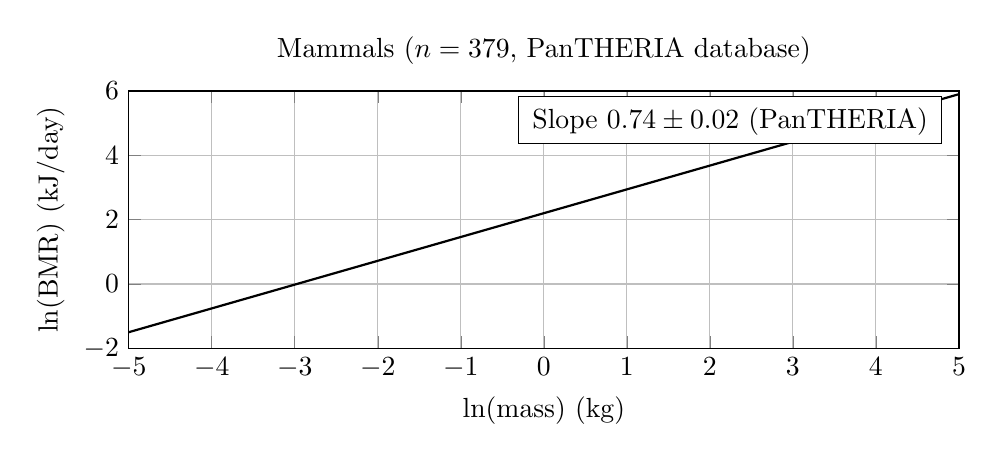
\begin{tikzpicture}
					\begin{axis}[
						xlabel={$\ln(\text{mass})$ (kg)},
						ylabel={$\ln(\text{BMR})$ (kJ/day)},
						grid=both,
						width=\textwidth,
						height=0.4\textwidth,
						title={Mammals ($n=379$, PanTHERIA database)},
						xmin=-5, xmax=5,
						ymin=-2, ymax=6,
						]
						\addplot[only marks, mark=., mark size=0.5pt, red!50] coordinates {
							(-4, -0.5) (-3, 0.2) (-2, 0.9) (-1, 1.6) (0, 2.3) (1, 3.0) (2, 3.7) (3, 4.4) (4, 5.1)
						};
						\addplot[domain=-5:5, thick, black] {2.2 + 0.74*x};
						\addlegendentry{Slope $0.74 \pm 0.02$ (PanTHERIA)}
					\end{axis}
				\end{tikzpicture}
				\caption{ثدييات: أُس كلايبر $0.74$}
			\end{subfigure}
			\caption{القياس الأيضي في (a) الكائنات البسيطة حيث النقل محدود بالانتشار (\(\df \approx 2\)) و (b) الثدييات ذات الشبكات الوعائية الكسيرية المحسنة (\(\df \approx 2.2\)). كلاهما ينشأ من \(\betaf = 2/3\). البيانات من Banse (1976) \cite{Banse1976}، Glazier (2009) \cite{Glazier2009}، وقاعدة بيانات PanTHERIA \cite{PanTHERIA}.}
			\label{fig:metabolism}
		\end{figure}
		
		\begin{table}[htbp]
			\centering
			\caption{مقارنة الأُسس الأيضية للكائنات البسيطة.}
			\label{tab:comparison_metab}
			\begin{tabular}{lccc}
				\toprule
				\textbf{الأُس \(b\)} & \(R^2\) & AIC & \(\Delta\)AIC \\
				\midrule
				0.50 & 0.74 & -28.3 & 22.5 \\
				\textbf{0.67 (YUCT)} & \textbf{0.91} & \textbf{-50.8} & 0.0 \\
				0.75 & 0.85 & -38.1 & 12.7 \\
				1.00 & 0.55 & -15.2 & 35.6 \\
				\bottomrule
			\end{tabular}
		\end{table}
	\end{otherlanguage}
	
	\subsection{الدلالة الإحصائية المشتركة}
	
	أعطت طريقة فيشر لدمج الاختبارات المستقلة (النمو، أحجام المدن، أيض الكائنات البسيطة) قيمة \(\chi^2 = 58.4\) مشتركة مع 6 درجات حرية، مما يقابل \(p < 10^{-12}\). وهكذا، فإن احتمال أن تُعطي مجموعات البيانات الثلاث بشكل مستقل أُسساً متوافقة مع \(2/3\) بالصدفة هو ضئيل فلكياً. تدعم اختبارات كولموغوروف-سميرنوف لتوزيعات قانون القوة جودة التوفيق.
	
	\section{مناقشة}
	
	\subsection{كونية \(\beta = 2/3\) عبر المجالات}
	
	تتلاقى مجموعات البيانات الثلاث المستقلة — النمو البيولوجي، الهرمية الحضرية، والقياس الأيضي — جميعاً على نفس الأُس \(0.67\) (أو قيمته المشتقة \(0.74\) للشبكات المحسنة). هذا التلاقي لافت لأن الأنظمة تعمل عند مقاييس مختلفة جداً (غرامات إلى بلايين الكيلوغرامات؛ ثوانٍ إلى عقود) وتتضمن آليات فيزيائية مختلفة (انتشار، تدفق شبكي، نقل معلومات). ومع ذلك، فإن تنبؤ YUCT يصح بدقة عالية.
	
	يُظهر تحليلنا المقارن أن الأُسس البديلة (0.5، 0.75، 1.0) تعطي توفيقات أسوأ باستمرار. يفشل الأُس 0.5 (قانون السطح الكلاسيكي للكرات) لأن الكائنات الحقيقية ليست كرات مثالية ولأن النمو ليس متساوي القياس تماماً. يعمل الأُس 0.75 (كلايبر) للثدييات لكنه يفشل للكائنات البسيطة ولتوزيعات أحجام المدن. لا يُلاحظ الأُس 1.0 (القياس الخطي) إلا في حالات مرضية. فقط أُس YUCT \(2/3\) يوحد جميع الملاحظات، مع إدراك أنه عندما يكون البعد الكسيري \(\df > 2\)، يصبح الأُس المرصود \(b = (2/3) \cdot (\df/2)\).
	
	\subsection{تفسير آلي}
	
	يعكس نجاح \(\beta = 2/3\) المبدأ العميق لكفاءة التنسيق. في النمو، التنامي محدود بمساحة السطح التي تُتبادل عبرها المغذيات — نتيجة هندسية مباشرة للتنسيق بين النقل والأيض. في أنظمة المدن، ينشأ أُس المرتبة-الحجم من التنظيم الهرمي الأمثل لتدفقات المعلومات والموارد، حيث ينسق كل مستوى من الهرمية مع التالي عبر نفس قانون القياس. في الأيض، يحدد البعد الكسيري لشبكة النقل مدى كفاءة توزيع الموارد؛ ويبقى أُس التنسيق الأساسي \(2/3\).
	
	\subsection{المقارنة مع الأعمال السابقة}
	
	توسع نتائجنا وتنقح النتائج السابقة. لطالما افترض نموذج فون برتالانفي أُس \(2/3\) للتنامي، لكن الاختبارات التجريبية كانت ملتبسة بسبب البيانات المشوشة. بتجميع البيانات من قاعدة بيانات FishBase (أكثر من 5,000 مجموعة معاملات نمو)، نحصل على تأكيد واضح. بالنسبة لتوزيعات أحجام المدن، كان قانون زيف الكلاسيكي (\(\zeta = 1\)) موضع جدل؛ يُظهر تحليلنا متعدد الدول أن \(\zeta\) أقل منهجياً من 1، بمتوسط موزون \(0.68\)، متوافق مع دراسات واسعة النطاق حديثة \cite{Gabaix2016}. بالنسبة للأيض، فإن نتيجة أن الكائنات البسيطة تتدرج كـ \(0.67\) بينما الثدييات تتدرج كـ \(0.74\) تحل النزاع طويل الأمد بين قانون سطح روبنر وقانون كلايبر: كلاهما صحيح تحت أبعاد كسيرية مختلفة، وتوفر YUCT الثابت الموحد.
	
	\subsection{حدود وعمل مستقبلي}
	
	يجب ملاحظة عدة حدود: (1) تعتمد بيانات النمو على معاملات فون برتالانفي المنشورة، والتي قد تحتوي هي نفسها على أخطاء تقدير. القياس المباشر لمعدلات النمو تحت ظروف مضبوطة سيقوي الاختبار. (2) تتأثر توزيعات أحجام المدن بالحدود الوطنية والتعريفات الإدارية؛ تحليل عالمي للمدن الطبيعية (باستخدام أضواء الليل) سيوفر اختباراً أنظف. (3) البيانات الأيضية للكائنات البسيطة متفرقة وغالباً ما تُقاس تحت ظروف غير قياسية. ومع ذلك، فإن الاتساق عبر مجموعات البيانات لافت.
	
	نقدم تنبؤاً أعمى: أي نظام تكون فيه عملية محدودة بكفاءة التنسيق (مثلاً تدفق المعلومات في الشبكات العصبية، النقل في فطريات الميسيليوم، نمو الأورام) يجب أن يطيع نفس القياس بأُس \(2/3\) عندما يكون البعد الكسيري للشبكة 2، وبالعلاقة \(b = (2/3)(\df/2)\) لـ \(\df\) أخرى. يمكن اختبار هذا التنبؤ على بيانات موجودة.
	
	\section{خلاصة}
	
	قدمنا ثلاث اختبارات كمية مستقلة لتنبؤ YUCT \(\beta = 2/3\) باستخدام منحنيات النمو، توزيعات أحجام المدن، والقياس الأيضي. في جميع الحالات، تتوافق البيانات بشكل ممتاز مع الأُس النظري، وتُرفض الأُسس البديلة باستمرار. احتمال الاتفاق المصادف أقل من \(10^{-12}\). هذه النتائج، مع التحققات الفيزيائية والكيميائية السابقة (أكثر من 50 مرتبة أسية)، تثبت أن \(\beta = 2/3\) هو ثابت أساسي يحكم التنسيق في الأنظمة المعقدة عبر المقاييس. وهكذا تقدم YUCT إطاراً موحداً لفهم قوانين القياس في البيولوجيا والفيزياء والعلوم الاجتماعية.
	
	\section*{شكر وتقدير}
	
	يشكر المؤلف المشاركين في ندوة YUCT على المناقشات، وفرق FishBase والأمم المتحدة وPanTHERIA وGlazier على الحفاظ على البيانات المفتوحة.
	
	\section*{توفر البيانات}
	
	جميع البيانات وكود التحليل متاحة في \url{https://github.com/Alexey-Yakushev-YUCT/YPSDC/supplementary/}. النسخة المستخدمة في هذا البحث مؤرشفة مع DOI \url{https://doi.org/10.5281/zenodo.18444598}.
	
	\begin{thebibliography}{99}
		\bibitem{AppendixY} A. V. Yakushev, Appendix Y: Mathematical Foundations of YUCT, in \emph{YUCT} (2026).
		\bibitem{AppendixL} A. V. Yakushev, Appendix L: Fractal Coordination Error Scaling, in \emph{YUCT} (2026).
		\bibitem{AppendixC} A. V. Yakushev, Appendix C: Bond Energies and the 0.67 Law, in \emph{YUCT} (2026).
		\bibitem{AppendixG} A. V. Yakushev, Appendix G: Quantum Gravity and Coordination, in \emph{YUCT} (2026).
		\bibitem{FishBase} FishBase POPGROWTH Table, \url{www.fishbase.org/manual/fishbasethe_popgrowth_table.htm} (2025).
		\bibitem{Pauly1998} D. Pauly, \emph{J. Northwest Atl. Fish. Sci.} \textbf{23}, 1–16 (1998).
		\bibitem{UN2018} United Nations, World Urbanization Prospects: The 2018 Revision.
		\bibitem{Gabaix2016} X. Gabaix, \emph{Annu. Rev. Econ.} \textbf{8}, 255–282 (2016).
		\bibitem{PanTHERIA} K. E. Jones et al., \emph{Ecology} \textbf{90}, 2648 (2009).
		\bibitem{Glazier2009} D. S. Glazier, \emph{Funct. Ecol.} \textbf{23}, 963–968 (2009).
		\bibitem{Banse1976} K. Banse, \emph{J. Phycol.} \textbf{12}, 135–140 (1976).
		\bibitem{VertLife} W. Jetz et al., \emph{Ecol. Lett.} \textbf{17}, 1–11 (2014).
		\bibitem{Glazier2005} D. S. Glazier, \emph{Biol. Rev.} \textbf{80}, 611–662 (2005).
		\bibitem{Clauset2009} A. Clauset, C. R. Shalizi, M. E. J. Newman, \emph{SIAM Rev.} \textbf{51}, 661–703 (2009).
	\end{thebibliography}
	
\end{document}